\chapter{Architecture}

The system architecture is shown in Figure~\ref{fig:architecture}. 
Apart from the HIP-VPLS switches, we have also implemented a unique 
control-plane protocol on top of the SSL protocol. 

%In our architecture, HIP switch controller is a central server instance that collects information from the HIP-switches
%and allows one to perform configuration of such parameters as firewall rules, HIP hosts file, MAC-based access
%controll lists (ACL) and configure traffic shaper. We are going to discuss each feature seperately 
%in the proceeding paragraphs.  

\begin{figure}[h!]
\centering
\includegraphics[width=0.7\textwidth]{graphics/arch.png}
\caption{System architecture}
\label{fig:architecture}
\end{figure} 

According to the protocol, on the one hand, every HIP-VPLS 
switch reports to the central controller (and is authenticated 
using the HMAC algorithm together with the shared symmetric 
master secret). In the implementation switches report their presence every $5$ 
seconds. On the other hand, every HIP-VPLS switch obtains 
the configuration from the central controller (such as mesh 
configuration, HIT resolver information, firewall rules, and 
MAC-based ACL). In the future, we also plan to support traffic 
shaper functionality.

Although we did not implement a traffic shaper feature in our 
HIP switches and HIP  controller, it is still valuable for future 
work. For example, different hosts can be served differently 
(with more bandwidth) than others by using traffic shaping. If 
some hosts in the HIP-VPLS network send delay-sensitive traffic, 
for example, curtain rules can be configured on the HIP controller 
to give a needed advantage over other hosts in the network. We 
leave this for future discussions and work.

In the testbed, we had a multihomed server (with one IP facing 
the public network so that HIP switches will be able to connect to 
the controller in the Internet, and one IP in the private range), 
several legacy microcomputers, IP camera, and DHCP/DNS server.


\chapter{Proof-of-a-concept implementation}
In this chapter, we will discuss the proof of a concept, or 
prototype, implementation of the HIP-VPLS (we will discuss 
how HIP-switches and controller were implemented). In our work, 
we have used the Python language as it offers simplicity at the 
cost of extra CPU cycles to do the job.

\begin{figure}[ht!]
\centering
\includegraphics[width=0.9\textwidth]{graphics/testbed.png}
\caption{Testbed setup}
\label{fig:testbed}
\end{figure}    

The experimental test-bed is shown in Figure~\ref{fig:testbed}. 
The source code for the HIP-VPLS infrastructure is available in 
the following repositories:~\cite{controllerimpl, hipswitchimp}.

Our prototype implementation consists of roughly 10K 
lines of code. Overall, the deployed architecture is 
shown in Figure~\ref{fig:architecture}. The communication 
between the HIP-VPLS switches is secured with HIP and IPSec 
protocols. The communication with the HIP-VPLS controller is 
secured with SSL protocol. We have chosen HIP protocol to 
secure the data-plane traffic as it does not rely on the 
TCP, hence reducing the wasted bandwidth and minimizing the 
delays (since IPSec does not rely on guaranteed delivery of a packet). 

The communication with the HIP-VPLS controller is authenticated 
using self-signed certificates. In addition, client authenticates 
itself to the controller using HMAC and preshared master secret. 
The format of the control packets can be looked up in the HIP 
controller source code found in our Git 
repository~\cite{controllerimpl}. 

To deploy the system, we have prepared the bash script. 
Overall, the deployment is trivial. The only things that 
need to change are the master secret and MySQL username 
and password. Otherwise, the administrator needs to execute 
the following commands in the server's console (observe, 
we have tested the deploy script on Ubuntu 22.04.2 LTS). 
So, to deploy the system, run the following (note that one 
needs to change the MySQL password in deploy.sh and config.py 
files (for both controller and configurator)):

\begin{verbatim}
$ git clone https://github.com/strangebit-io/hip-vpls-controller.git
$ cd hip-vpls-controller/deployment
$ sudo bash deploy.sh
\end{verbatim}

After the HIP controller and configurator are deployed, 
one needs to deploy the HIP switch code on NanoPI R2S 
(remember you need to copy the certchain.pem - self-signed 
certificates and change the master secret to match the one 
specified for the HIP controller. Also, the administrator 
needs to change the public, routable on the Internet, 
IP address in the configuration and specify the switch name):


\begin{verbatim}
$ git clone https://github.com/strangebit-io/hip-vpls-hw-with-controller.git
$ cd hip-vpls-hw-with-controller/
$ sudo bash deployment/deploy.sh
\end{verbatim}

One important aspect. The clocks on NanoPI R2S must be set to UTC and 
synchronized with the controller (otherwise, certificate verification 
will fail during the SSL handshake).

Once everything is set, open the browser and open the location 
http://192.168.1.3:10000/ (or, whatever the IP address of the HIP 
controller node is, this needs to be routable in the Internet IP 
address). One should see the following screen (see 
Figure~\ref{fig:login}). The credentials can be found in the 
schema.sql file in the database folder. 

\begin{figure}[h!]
\centering
\includegraphics[width=0.9\textwidth]{graphics/login_screen.png}
\caption{Prototype: login screen}
\label{fig:login}
\end{figure}

After successful login, the device status page will open. Here, 
all registered (registration is performed automatically) HIP 
switches will appear. One can check the status, HIT, and IP of the 
switches.

\begin{figure}[ht!]
\centering
\includegraphics[width=0.9\textwidth]{graphics/devices.png}
\caption{Prototype: devices status information}
\label{fig:devices}
\end{figure}
\clearpage

Next, one needs to configure the mesh for a distributed network. 
In our setup, we listed all possible pairs of HIP-switches. That 
is the typical configuration option. For example, see Figure~\ref{fig:mesh}.

\begin{figure}[h!]
\centering
\includegraphics[width=0.9\textwidth]{graphics/mesh.png}
\caption{Prototype: mesh configuration}
\label{fig:mesh}
\end{figure}
\clearpage

Then, one needs to specify the HIP firewall rules. This operation 
should be done on the firewall tab. See Figure~\ref{fig:firewall}. 
Again, a typical setup should have all pairs of HITs.

\begin{figure}[h!]
\centering
\includegraphics[width=0.9\textwidth]{graphics/firewall.png}
\caption{Prototype: HIP firewall}
\label{fig:firewall}
\end{figure}
\clearpage

The final step is to configure MAC address-based access control 
(see Figure~\ref{fig:mac}). Here, one needs to specify (in the 
outgoing direction) the necessary MAC address pairs of hosts in 
the network. Remember that this step needs to be completed for 
each HIP switch separately.

\begin{figure}[h!]
\centering
\includegraphics[width=0.9\textwidth]{graphics/MAC-ACL.png}
\caption{Prototype: MAC address based access control lists}
\label{fig:mac}
\end{figure}
\clearpage

%\begin{figure}[h!]
%\centering
%\includegraphics[width=0.9\textwidth]{graphics/reg_packet.png}
%\caption{Registration packet}
%\label{fig:reg_packet}
%\end{figure}

%\section{Accelerating AES with the hardware}

Overall, we were not satisfied with the HIP switches. We were observing 
roughly $120 Kbits/s$ throughput using the IPerf tool. 

\begin{figure}[h!]
\centering
\includegraphics[width=0.9\textwidth]{graphics/AES.pdf}
\caption{AES encryption performance}
\label{fig:aes}
\end{figure}

So we have tried to improve the performance by implementing in C++ and assembly language
AES256 cryptographic algorithm. Luckily, the NanoPI R2S chip (ARM Cortex 
53) supports the AES256 instruction set. We have cross-compiled the 
library and used it in our HIP switch implementation. The results for AES256 
encryption is shown in Figure~\ref{fig:aes}. The performance of AES256 
implemented with special CPU instructions was ten times faster. Thus, our 
preliminary experiments showed that we can achieve maximum $2.4 Mbits/s$ 
throughput between pair of hosts (the entire distribution is shown in Figure~\ref{fig:tput}).


\begin{figure}[h!]
\centering
\includegraphics[width=0.9\textwidth]{graphics/iperf.pdf}
\caption{Throughput performance}
\label{fig:tput}
\end{figure}



We have also performed tests on more productive Intel N95 CPUs. The test scenario is show in Figure~\ref{fig:test}.
We have bought 3 mini-PCs with N95 Intel CPU (running at 3.4GHz in turbobust regime). We have used speedtest library 
to test the connection (download and upload) with the server in the Internet. The results for the SHA256-HMAC with NULL
cipher and SHA256-HMAC with AES256 are depicted on Figure~\ref{fig:results}.

\begin{figure}[h!]
\centering
\includegraphics[width=0.9\textwidth]{graphics/test.png}
\caption{Test configuration}
\label{fig:test}
\end{figure}

Some simple statistics from the data: Mean download throughput (Mbits/s) for NULL cipher (29.86796),
mean upload throughput for NULL cipher(23.34449), mean download throughput (Mbits/s) for AES256 (25.2982),
and finally, mean upload throughput for AES256 cipher(19.9534).

\begin{figure}[h!]
\centering
\includegraphics[width=0.9\textwidth]{graphics/final.pdf}
\caption{Download and upload speeds for NULL cipher and AES256 (hardware accelerated)}
\label{fig:results}
\end{figure}

